\chapter{Data}

\section{Data Description}

The data used in this thesis can be split into two portions: the economic data and the market returns.

\subsection{Data Origin}

The economic data is retrieved from the Jensen, Kelly, and Pedersen dataset. The dataset includes a comprehensive collection of equity market factors described in their paper "Is There a Replication Crisis in Finance?" (2023). The data is publicly available with extensive documentation of factor definitions and construction methods. The JKP factors are constructed using data from the Center for Research in Security Prices (CRSP), Compustat, I/B/E/S, and OptionMetrics. The data is available for both the U.S. economy and the Chinese economy.

The market data is retrieved from Finaeon, a platform that provides financial and economic data, including over 307,000 global data series spanning markets from 1000 AD to the present. They compile their data from a variety of historical and current sources, including financial reports, news periodicals, sectoral journals, and other publications, all of which are meticulously transcribed and verified.

\subsection{Factor Data}

Data is provided on 153 unique factors representing the U.S. and Chinese economies, measured at both a daily and monthly granularity. The factors are value-weighted by a method called \textit{capped market capitalization}, meaning that the impact of a company on the measure is weighted by its size, winsorized at the 80th percentile level. Using market capitalization as a weight is standard in the market as it better reflects investable opportunities and is less volatile than equally-weighted values. The capping methodology is implemented by JKP to cap the impact a singular company can have on the measure to 80\%.

The factors can be split into the following categories: enterprise value, earnings momentum, earnings quality, sales growth, volatility measures, liquidity, market size, and technical factors like Amihud illiquidity and maximum returns. 

The U.S. monthly data has 1,188 rows and covers January 1926 to December 2024; of those, 638 include measurements of all 153 factors. The U.S. daily data has 26,051 rows and covers January 2, 1926 to December 31, 2024; of those, 13,407 have measures of all 153 factors.

The Chinese monthly data has 348 rows and covers November 1993 to December 2024; of those, 112 include measurements of all 153 factors. The Chinese daily data has 7,109 rows and covers November 1, 1993 to December 31, 2024; of those, 2,266 have measures of all 153 factors.

\subsection{Themes Data}

The U.S. and Chinese factor data are provided as 13 themes, each aggregating multiple factors; as such, the theme data is also value-weighted by market capitalization. The theme data is available at a daily and monthly granularity. The themes are: accruals, debt issuance, investment, low leverage, low risk, momentum, profit growth, profitability, quality, seasonality, short term reversal, size, and value. Descriptions for each of these themes are provided below.

\begin{description}
   \item[Accruals] Measures the difference between a company's reported earnings and its cash flows. Lower values signal a higher quality of sustainable earnings. 
   \item[Debt Issuance] Tracks changes in corporate debt.
   \item[Investment] Measures corporate spending on assets, capital expenditures, and acquisitions. 
   \item[Low Leverage] Measures absolute debt levels. 
   \item[Low Risk] Captures stocks with lower risk measures, often represented by volatility.
   \item[Momentum] Measures return persistence and trend-following behavior.
   \item[Profit Growth] Measures change in profit margins and earnings.
   \item[Profitability] Measures levels of corporate profitability.
   \item[Quality] Combines measures of financial stability, earnings consistency, governance, and operational efficiency. 
   \item[Seasonality] Captures recurring calendar-based patterns in market returns.
   \item[Short Term Reversal] Measures the tendency of stocks to reverse their previous 1-4 week performance. 
   \item[Size] Measures market capitalization, allowing to distinguish between company sizes.
   \item[Value] Identifies stocks trading at lower prices relative to their values of fundamental measures (book value, earnings, cash flows, or sales). 
\end{description}

The U.S. monthly data has 1,188 rows and covers January 1926 to December 2024; of those, 878 include measurements of all 13 themes. The U.S. daily data has 26,051 rows and covers January 2, 1926 to December 31, 2024; of those, 18,443 have measures of all 13 themes.

The Chinese monthly data has 348 rows and covers November 1993 to December 2024; of those, 336 include measurements of all 13 themes. The Chinese daily data has 7,109 rows and covers November 1, 1993 to December 31, 2024; of those, 6,787 have measures of all 13 themes.

\subsection{Market Returns}

The Wilshire 5000 Total Market Index and the Shanghai SE Composite were chosen to represent the equity markets in the U.S. and China, respectively, because of their broad coverage of the markets. The Wilshire 5000 is a market-capitalization-weighted index of the market value of all American stocks actively traded in the United States. The Shanghai SE Composite is an index of all stocks traded at the Shanghai Stock Exchange.

The data is available at the daily and monthly levels. The Wilshire 5000 data dates back to 1970 and is available until May, 2024, and the Shanghai Composite data dates back to its opening in 1990 and is available until December, 2024. 

The close values at the end of the market day are used. The returns are also given as percent changes from the previous period, either daily or monthly. The Shanghai Composite is given in U.S. dollars.

\section{Exploratory Data Analysis}
\subsection{Data Cleaning}

The data was provided in high quality, as JKP cleaned the data before publishing it. The market data provided by Finaeon was also of great quality, which is expected as they are providers of data for financial researchers and professionals. Most of the data was provided in a stacked format. After pivoting the datasets, I analyzed it for missingness and temporal coverage. While the missingness and temporal coverage are explored for the entire dataset, the trends are explored for 2001 to 2024, the data available after China joined the World Trade Organization. 

\subsection{Data Trends}
\subsubsection{Market Trends}

Data trends are explored on a monthly granularity to reduce the impact of noise. Looking at the market returns for the U.S. and China, shown in Figure~\ref{fig:label1}, we see that the Chinese market is much more volatile than the U.S. market.

\begin{figure}[htbp]
\begin{center}
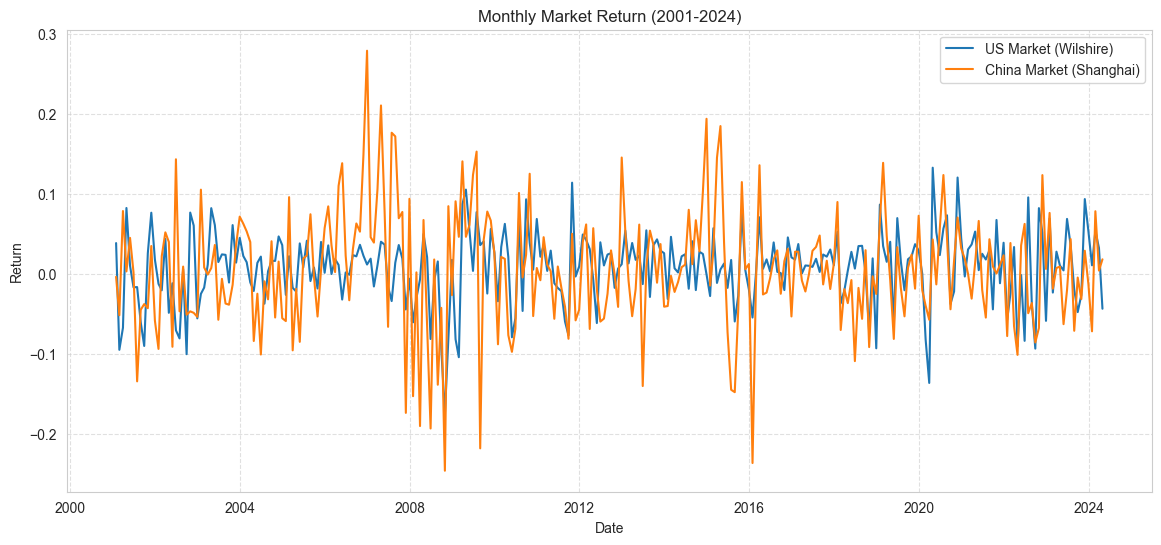
\includegraphics[width=4in]{figures/trends/Monthly Market Returns.png}
\caption{Monthly Market Returns}
\label{fig:label1}
\end{center}
\end{figure}

Even after calculating the 6-month moving average, displayed in Figure~\ref{fig:label2}, the volatilities are clearly different. Note that the greatest differences appear around the 2005-2008 period, the 2014-2016 period, and the 2018-2019 period. 

\begin{figure}[htbp]
\begin{center}
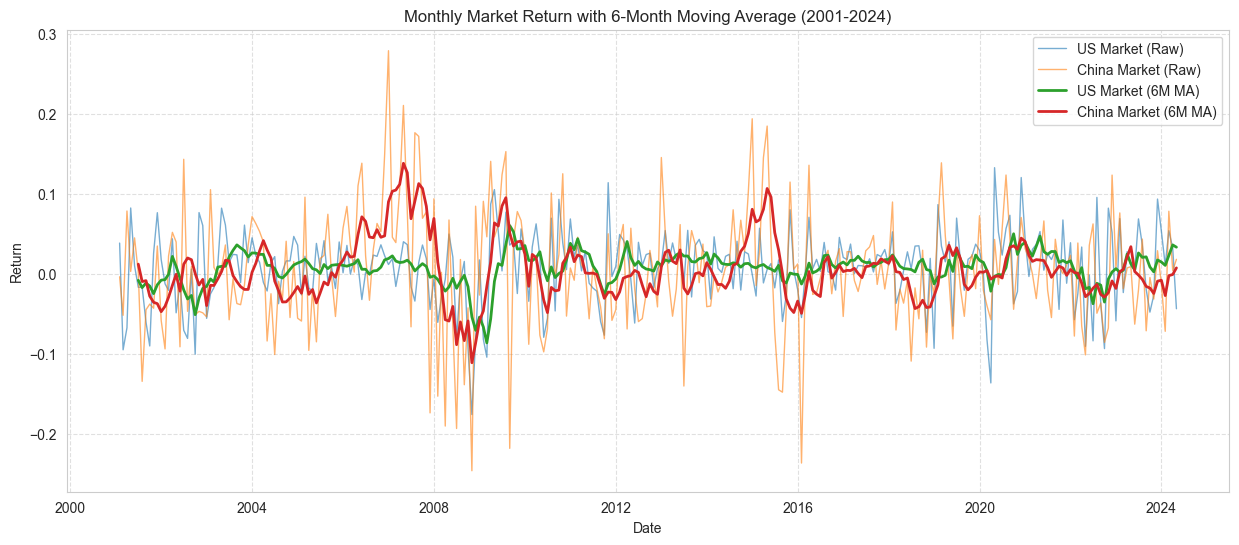
\includegraphics[width=4in]{figures/trends/Monthly Market Returns with Moving Average.png}
\caption{Monthly Market Returns with 6-Month Moving Averages}
\label{fig:label2}
\end{center}
\end{figure}

During the 2005-2008 period, China's economy experienced rapid growth and market liberalization. This explains the period of higher returns that was not exhibited in the U.S. market. The 2008-2010 period had similar impacts on the U.S. and China as financial crises led to sharp market corrections in both markets. In the U.S., the markets were crashing because of the bursting of the housing bubble and the failures of the financial sector. In China, investors fear surrounding the slowing exports and accumulated debt led to a market correction. 

The 2014-2016 period had large increases and decreases in returns in China, while the U.S. economy remained relatively stable. The trends in China were mainly due to the retail bubble and its burst.

In 2018-2019, the Chinese market corrected after growing too quickly. 

\subsubsection{Economic Trends}
Economic trends are explored at the monthly level once again to avoid volatility and noise. Themes are visualized for greater explainability as there are 13 themes and 153 factors. 

The 6-month moving averages of the 13 themes are plotted in Figure~\ref{fig:label3} from 2001 to 2024 to reduce noisy peaks and increase visibility in trends. We notice, consistent with the market data, that the Chinese economy is less stable than the U.S. economy, with themes generally being more volatile. 

\begin{figure}[htbp]
\begin{center}
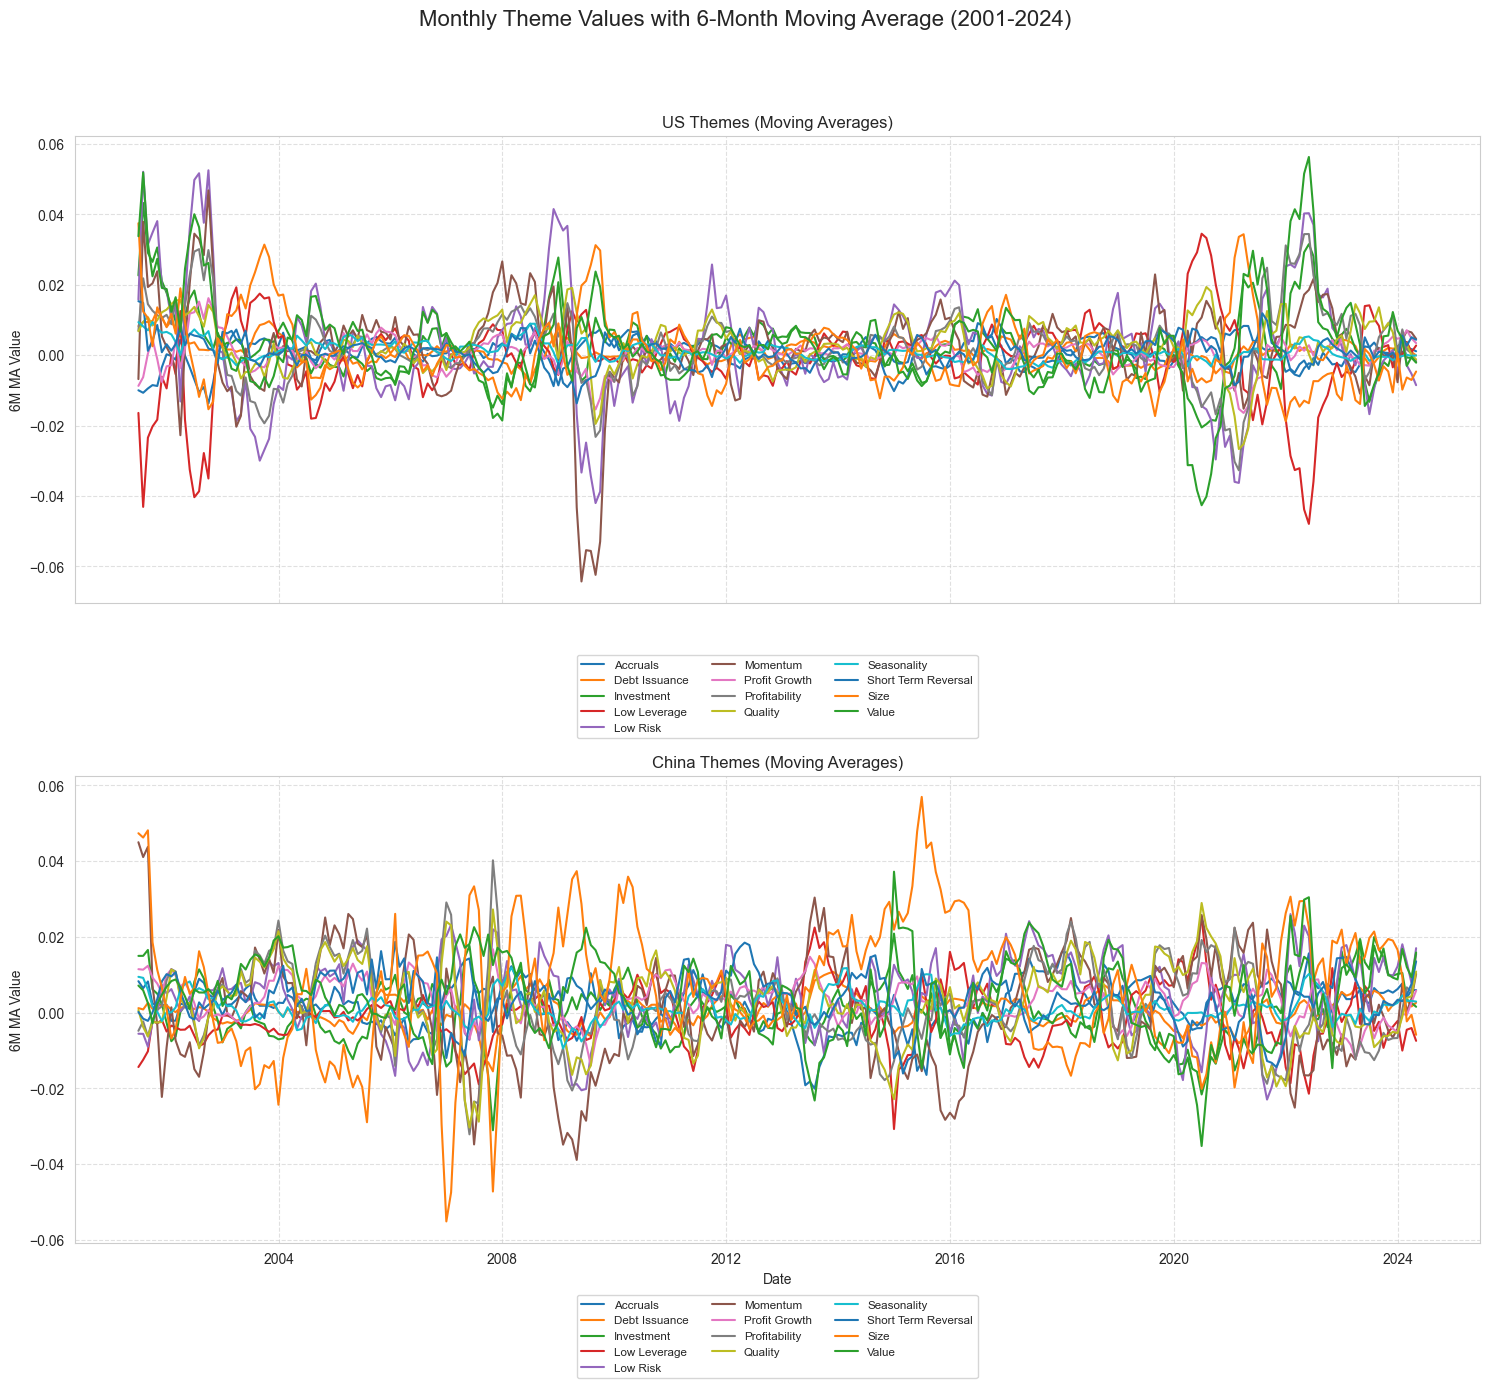
\includegraphics[width=5in]{figures/trends/Monthly Theme Moving Average Values.png}
\caption{Monthly Theme 6-Month Moving Averages}
\label{fig:label3}
\end{center}
\end{figure}

We do also notice general trends between the market returns and the economic themes within countries as periods with high volatility in markets typically align with high volatility in economic themes.

\subsection{Correlations and Collinearity}

Themes correlations are analyzed using a correlation heatmap, shown in Figure~\ref{fig:label18} for the U.S. and in Figure~\ref{fig:label19} for China. Note that there appear to be several strong correlations in the U.S. and Chinese data, but the correlations are not necessarily the same for both countries. Some of the strongest correlations in the U.S. market are uncorrelated in the Chinese market, and vice versa. This implies that the markets have structural differences, and that the themes important for market signals in the U.S. might not be important signals for the Chinese market.

\begin{figure}[htbp]
\begin{center}
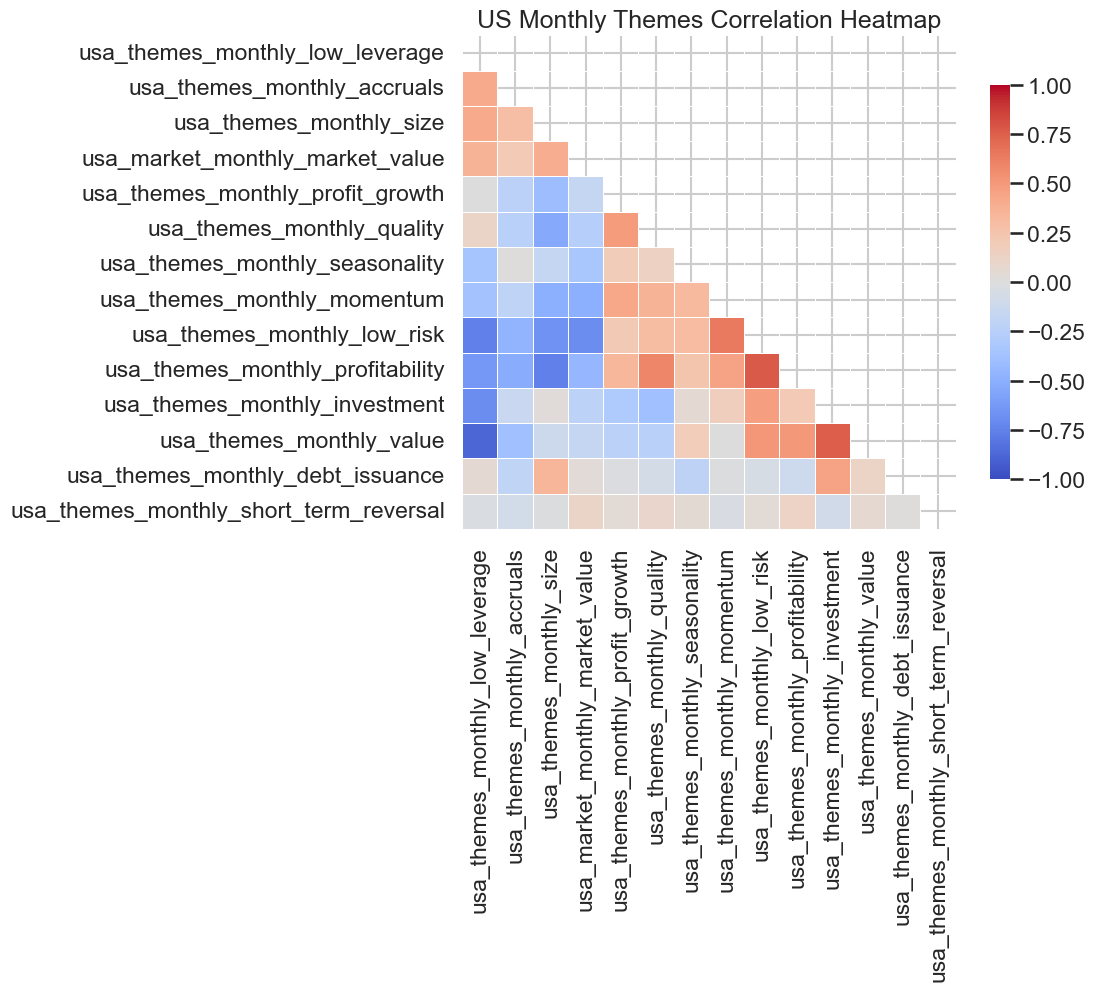
\includegraphics[width=4in]{figures/correlations/US Monthly Themes Correlation Matrix.png}
\caption{U.S. Monthly Themes Correlation Heatmap}
\label{fig:label18}
\end{center}
\end{figure}


\begin{figure}[htbp]
\begin{center}
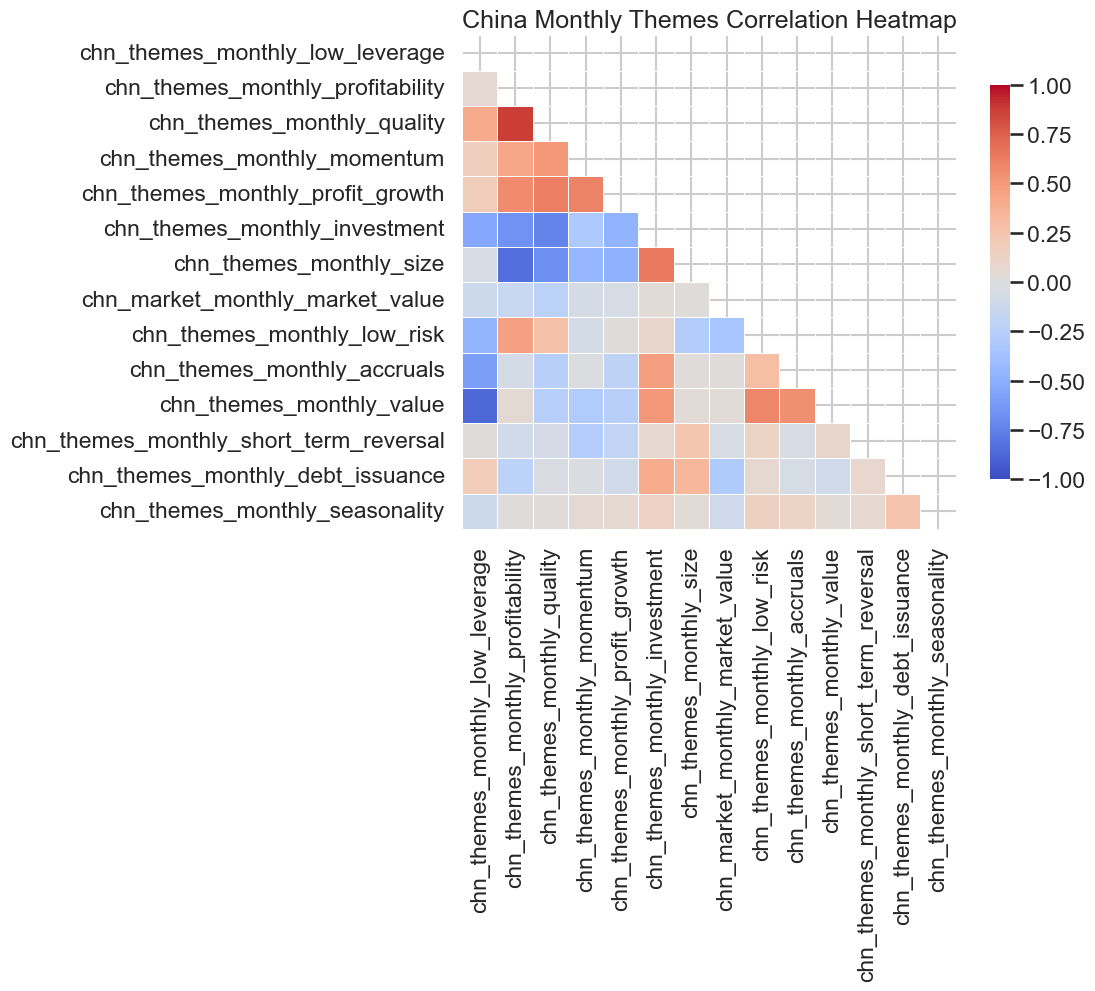
\includegraphics[width=4in]{figures/correlations/China Monthly Themes Correlation Matrix.png}
\caption{China Monthly Themes Correlation Heatmap}
\label{fig:label19}
\end{center}
\end{figure}

Correlation networks were also analyzed in the U.S. and China Themes and Factors datasets at a daily granularity. The themes network in the U.S., shown in Figure~\ref{fig:label20}, reveals only correlations ($r\geq 0.70$) among the low leverage, value, and investment themes. The themes network in China, shown in Figure~\ref{fig:label21}, reveals a similar trend in which value and low leverage are correlated ($r\geq 0.70$). It also shows that, in China, size is correlated to profitability, profitability is correlated to quality, and quality is correlated to investment. Figure~\ref{fig:label22} and Figure~\ref{fig:label23} show the factor correlation networks for the U.S. and China, respectively.

\subsection{Missingness}

\subsubsection{Factor Data}
While some U.S. factors have data points as early as 1926, they only comprise 29 of the 153 factors. Data is available for 40 factors starting in 1930, 49 factors starting in 1950, 136 factors starting in 1960, and all 153 factors are available after 1972. These trends for missing values in the daily and monthly factors for U.S. data are shown in the top subplot in Figure~\ref{fig:label4}.

For the Chinese factors, we see a similar decreasing trend, in which more data is available for more recent years. However, the Chinese data availability is much more volatile. Note that the data is much more stable post 2001, the year in which China joined the WTO. This is typically the earliest that the literature begins considering China a liberalized market, and is the earliest data that will be included in our models. These trends for missing values in the daily and monthly factors for China data are shown in the bottom subplot in Figure~\ref{fig:label4}.

\begin{figure}[htbp]
\begin{center}
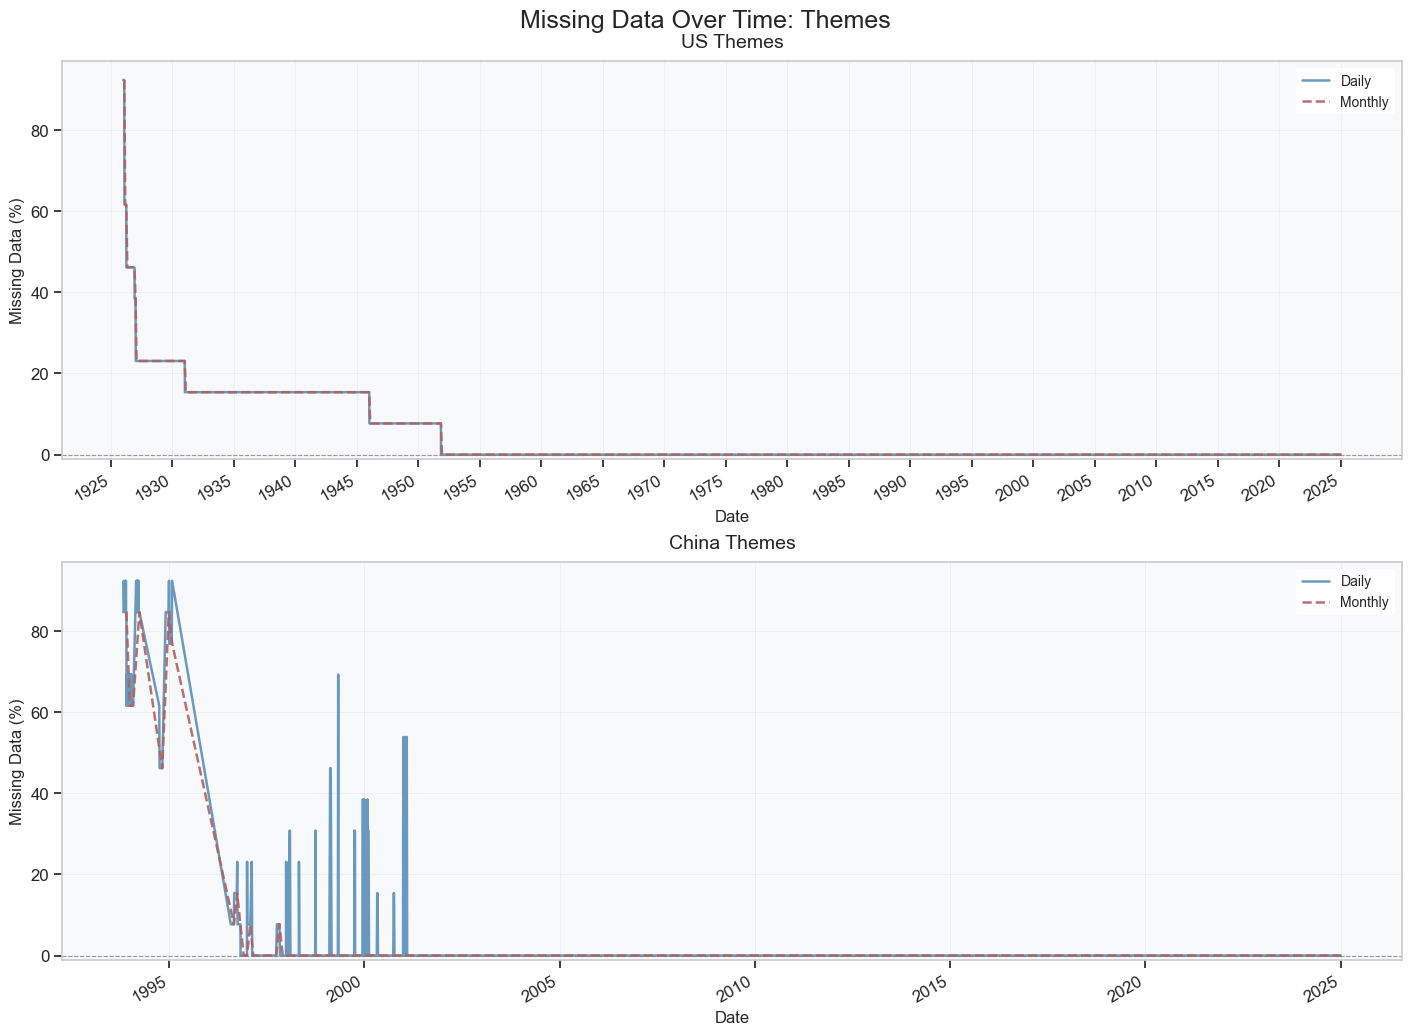
\includegraphics[width=5in]{figures/missingness/Themes Missing Data.png}
\caption{Factors Missing Values Over Time}
\label{fig:label4}
\end{center}
\end{figure}

\subsubsection{Themes Data}

The U.S. themes data is much more available, with no missingness after 1960 in either the daily data or the monthly data. These are shown in the top subplot in Figure~\ref{fig:label5}.

The Chinese daily themes are still volatile before 2002 in terms of missingness, but the monthly data is complete from 1999 onward. These trends are shown in the bottom subplot in Figure~\ref{fig:label5}.

\begin{figure}[htbp]
\begin{center}
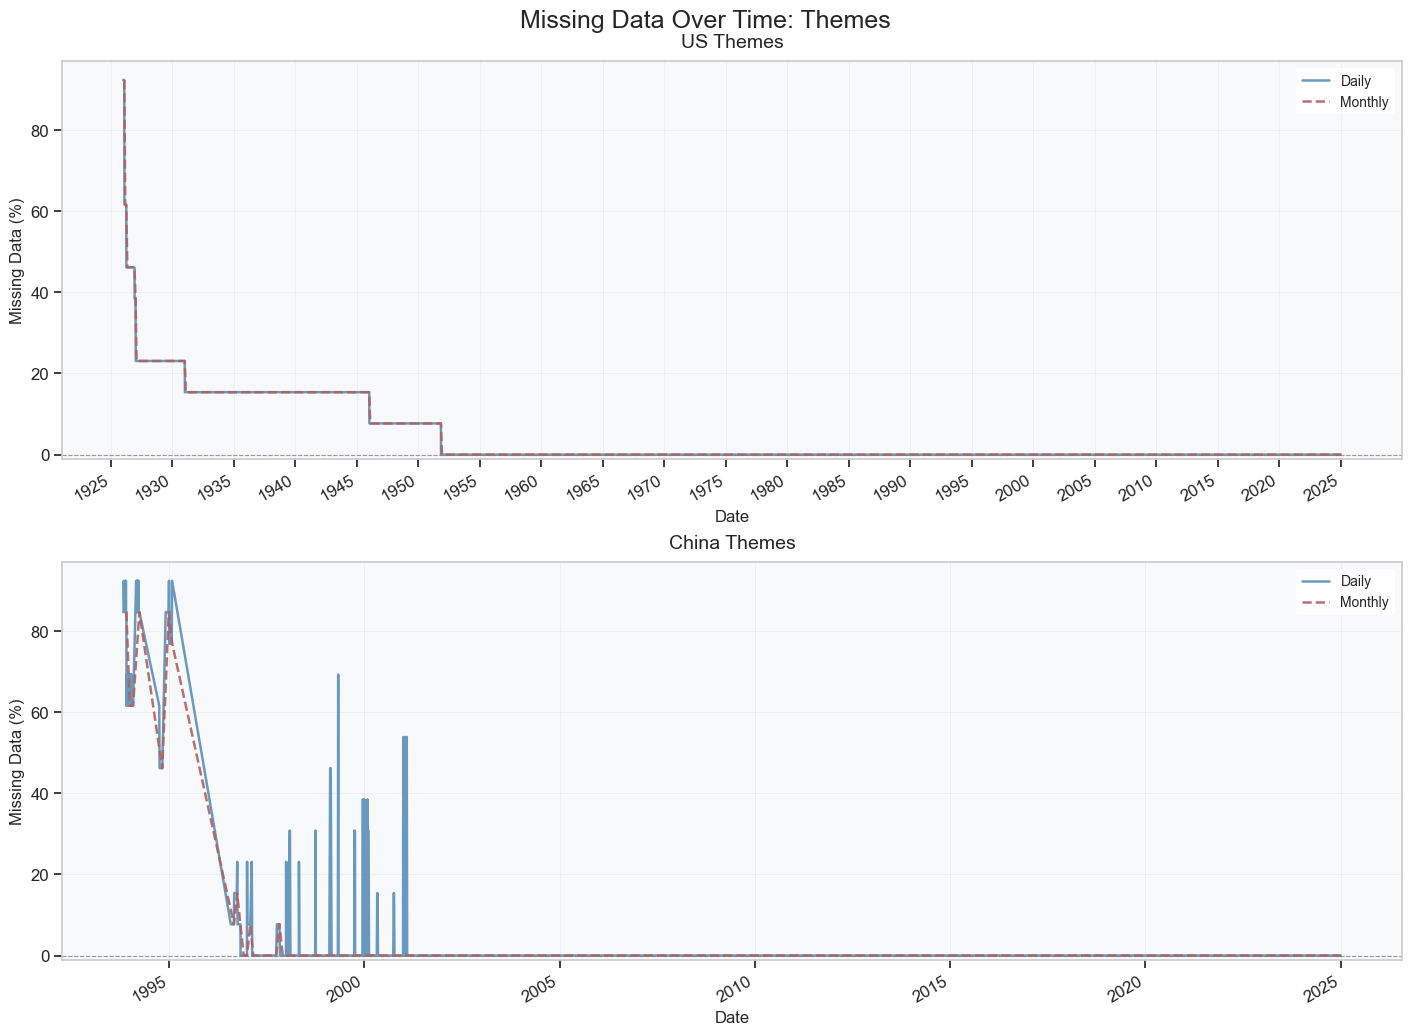
\includegraphics[width=5in]{figures/missingness/Themes Missing Data.png}
\caption{Themes Missing Values Over Time}
\label{fig:label5}
\end{center}
\end{figure}

A few trends come out in the missingness of the data. First, data missingness is generally decreasing over time. Second, themes data is more complete than the factors, with no missingness after 1960 for the U.S. and 2002 for China. Third, data with monthly granularity tends to have less missingness than daily data with daily granularity.

\subsubsection{Handling Missingness}

The monthly themes data does not exhibit any missingness in the data. The daily themes, on the other hand, have some sporadic missingness in the data. Figure ~\ref{fig:label13} shows the missingness observed in the daily themes for the 40 themes with the most missingness. The missingness is sporadic, and will be imputed using linear imputation.

\begin{figure}[htbp]
\begin{center}
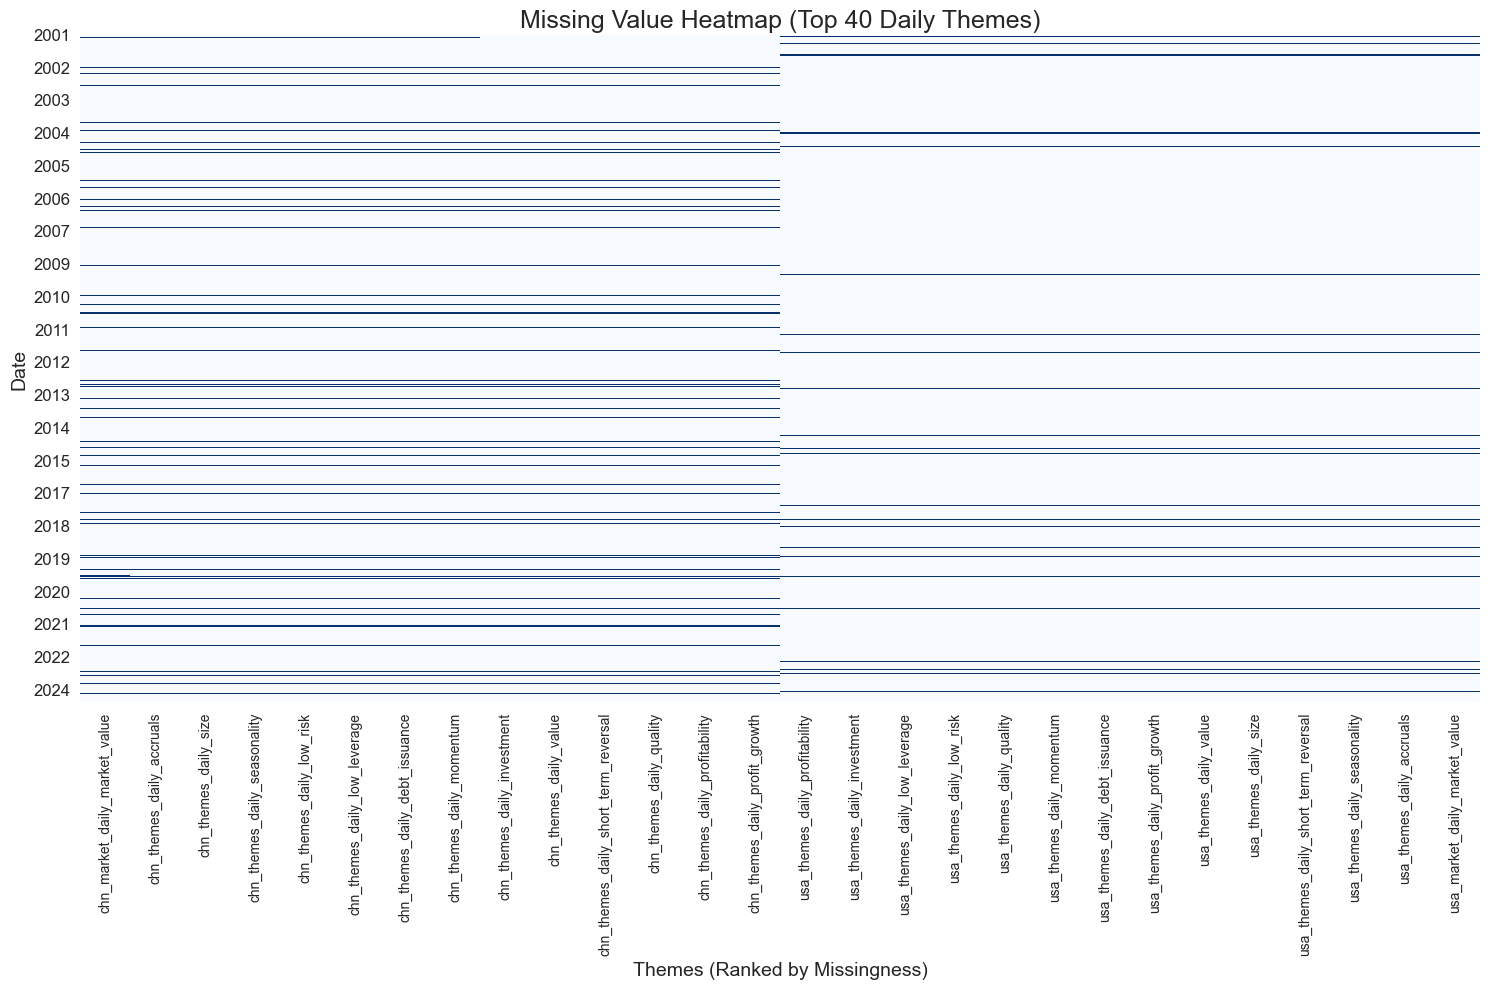
\includegraphics[width=5in]{figures/missingness/Themes Daily.png}
\caption{Missing Themes Heatmap (Top 40 Themes, Daily Data)}
\label{fig:label13}
\end{center}
\end{figure}


The factor data, on the other hand, exhibits much more severe missingness. Figure ~\ref{fig:label14} shows the 40 factors with the most missingness on a daily factor. The missingness can be decomposed into two types: (1) sporadic missingness similar to that observed with the daily themes data, which can be linearly imputed, and (2) large chunks of missing data for some of the Chinese factors. These factors, listed below and shown in Figure ~\ref{fig:label14}, have too much missing data to be considered, often not having any data for the first 4-13 years of the data. In order to avoid bias, I've excluded the factors from both countries' data.

The factors I've excluded from the data are: rd5\_at, seas\_16\_20an, seas\_16\_20na, rd\_me, rd\_sale, emp\_gr1, sale\_emp\_gr1, seas\_11\_15an, seas\_11\_15na, seas\_6\_10na, seas\_6\_10an, iskew\_hxz4\_21d, ivol\_hxz4\_21d, ocfq\_saleq\_std, saleq\_su, eqnetis\_at, saleq\_gr1, ni\_inc8q, capex\_abn, capx\_gr3, resff3\_6\_1, resff3\_12\_1, niq\_su.

Figure ~\ref{fig:label15} shows the missingness on the monthly level, which is similar to the daily plot in Figure ~\ref{fig:label14} but without the dates where data is missing for all factors. The same factors are excluded from the monthly data.

\begin{figure}[htbp]
\begin{center}
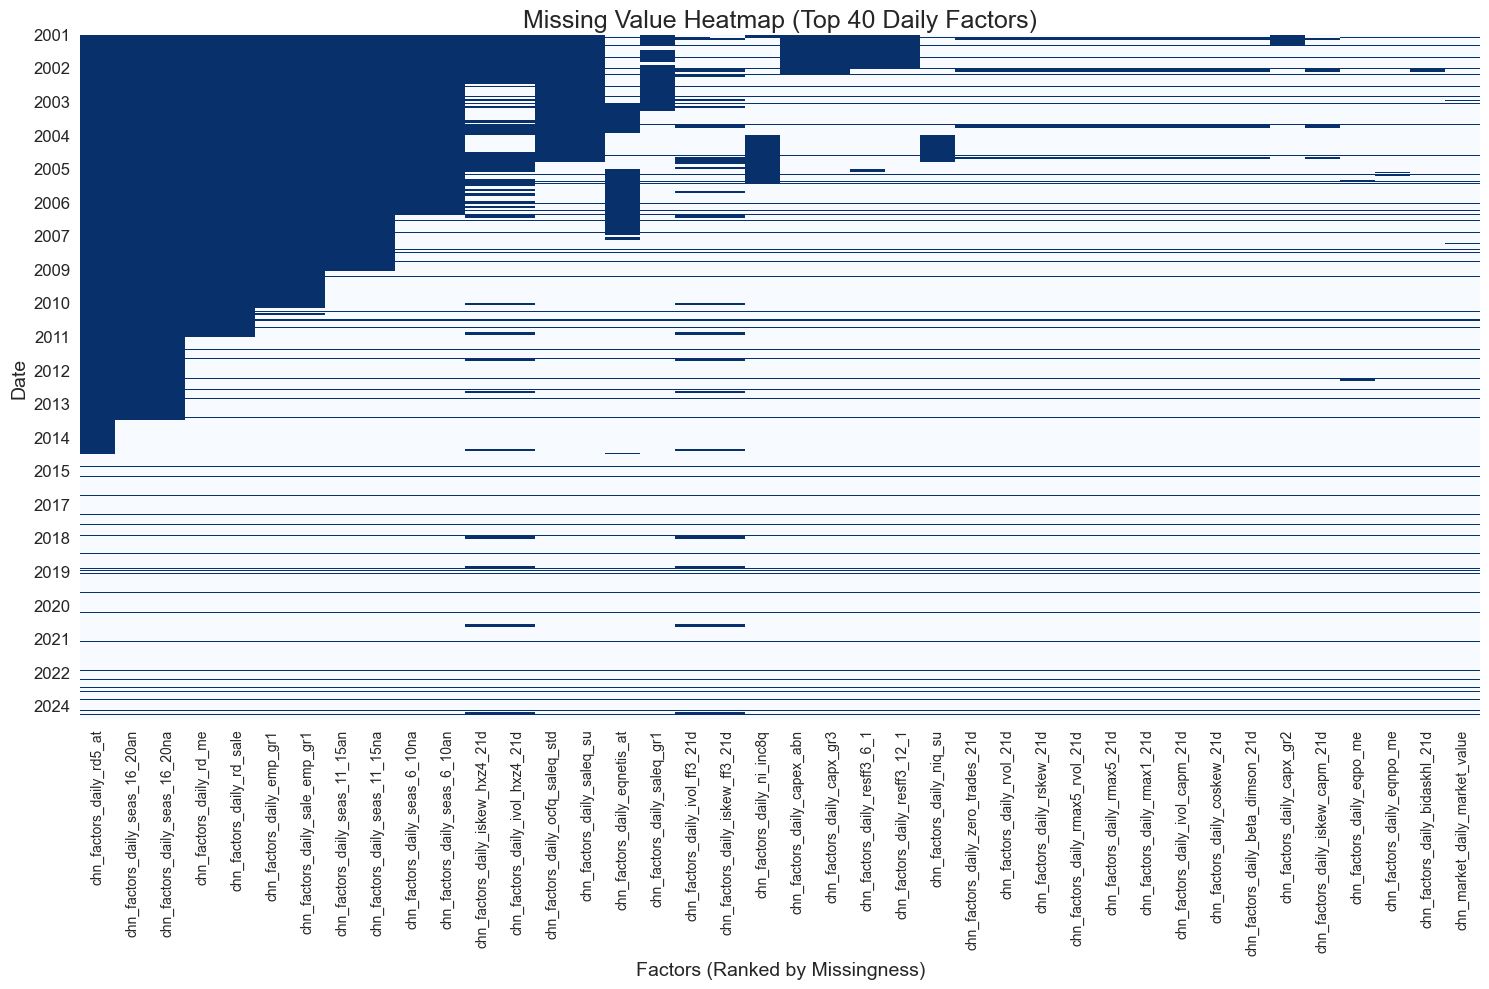
\includegraphics[width=5in]{figures/missingness/Factors Daily.png}
\caption{Missing Factors Heatmap (Top 40 Factors, Daily Data)}
\label{fig:label14}
\end{center}
\end{figure}


\subsubsection{Market Returns Data}

While no missingness was initially exhibited in the data at either the daily or the monthly granularity, further analyses showed some gaps in temporal coverage at the daily granularity. Figure~\ref{fig:label6} shows the gaps. Gaps were calculated as periods of more than two business days without data for the daily level and any month without data for the monthly level. Gaps do not account for federal holidays or other yearly missingness in the data. This is not central to the analyses, so it was not explored in more depth. The largest gaps are shown, with 23 business days in the U.S. daily data and 14 business days in the Chinese daily data.

Additionally, there were some days where the markets were closed but the factor and theme data were available. I chose to omit these from the data since the observed outcome is not measured.

\begin{figure}[htbp]
\begin{center}
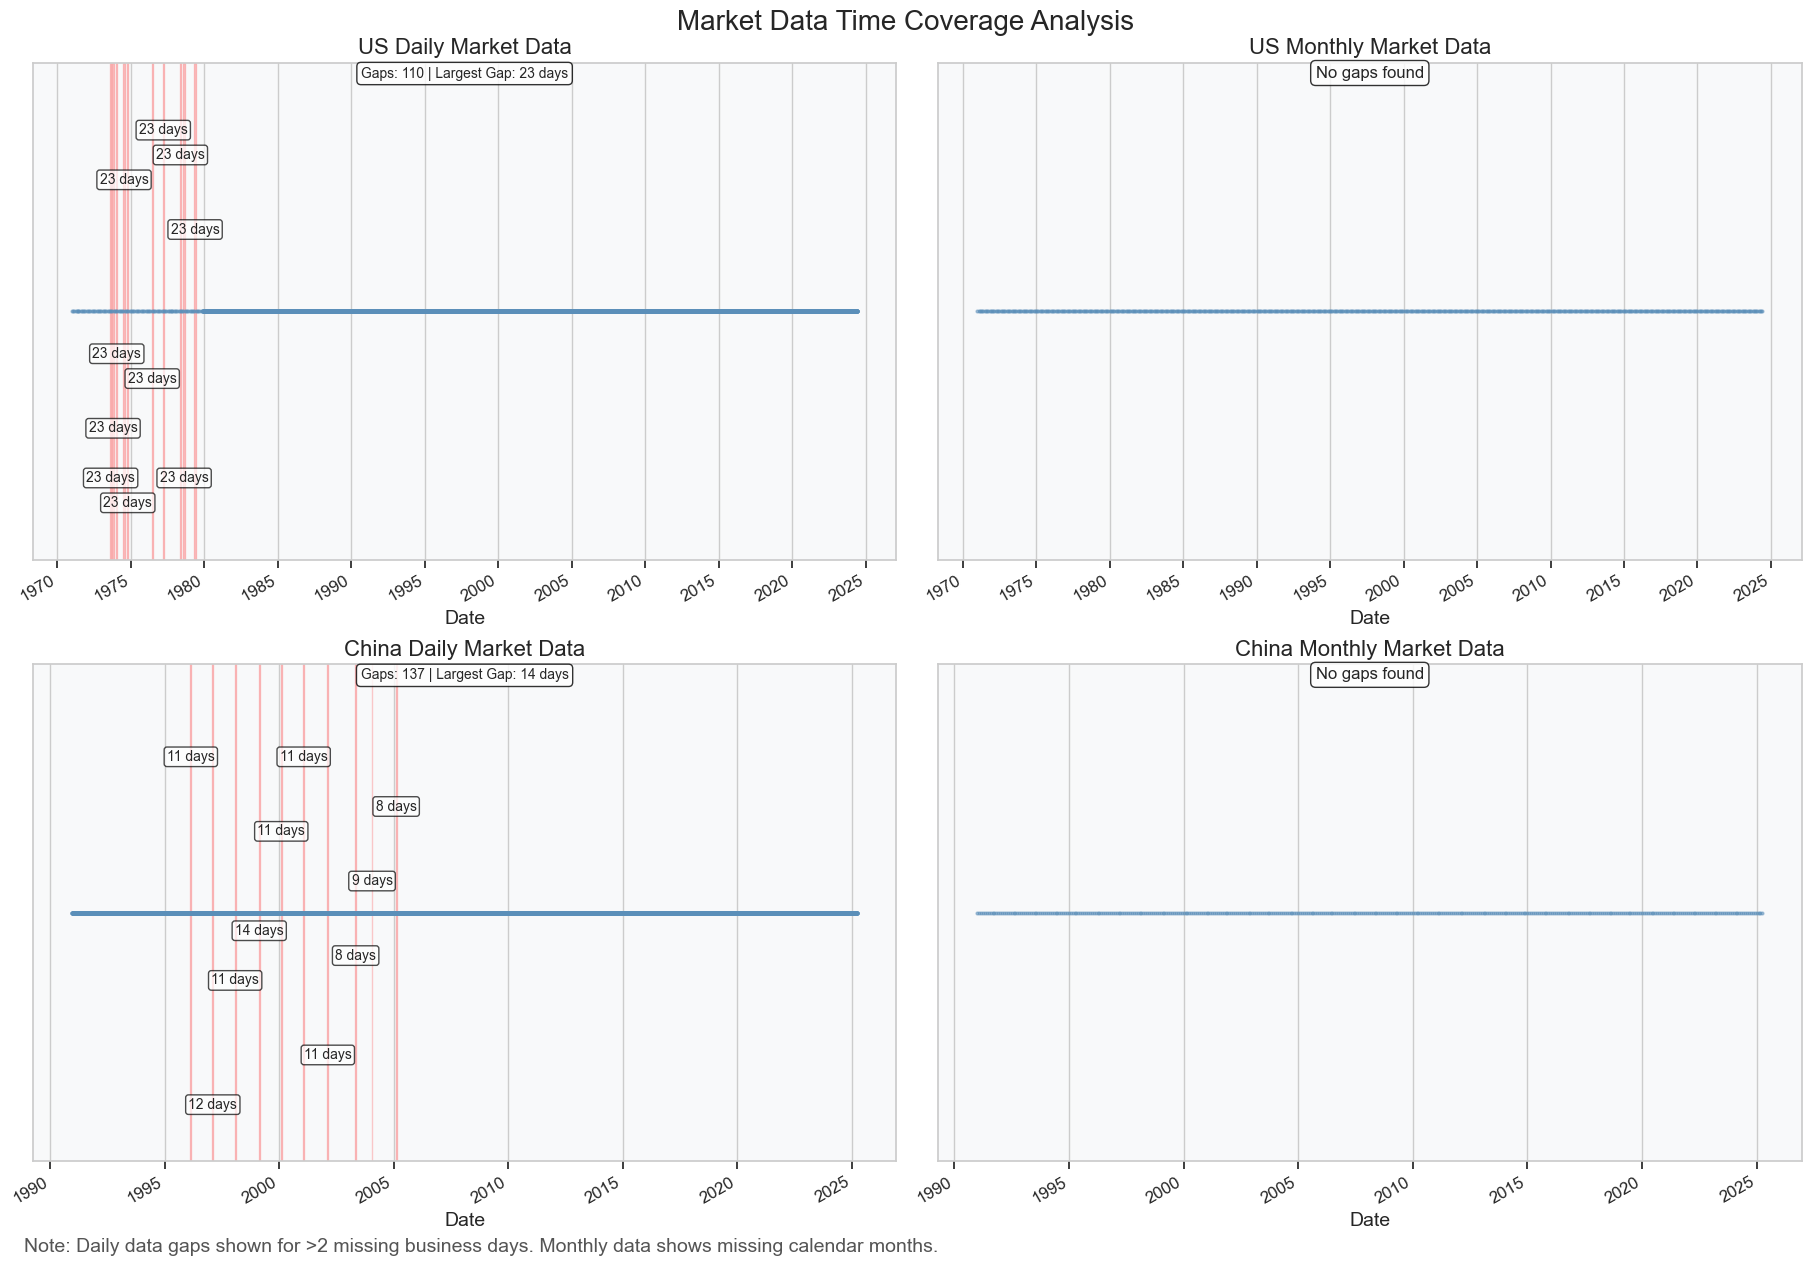
\includegraphics[width=5in]{figures/missingness/Market Data Coverage.png}
\caption{Market Data Time Coverage Analysis}
\label{fig:label6}
\end{center}
\end{figure}

\subsection{Consistency and Outlier Analysis}
\subsubsection{Market Outliers}

I first merged the data to create four Pandas dataframes: (1) Factors with Market Returns for the U.S. and China at a daily granularity, (2) Factors with Market Returns for the U.S. and China at a monthly granularity, (3) Themes with Market Returns for the U.S. and China at a daily granularity, and (4) Themes with Market Returns for the U.S. and China at a monthly granularity.

Using the IQR method, 6 outliers were detected in the U.S. market returns and 11 outliers were detected in the Chinese market returns. Figure~\ref{fig:label7} shows the dates that the outliers appeared. Of the 17 total outliers, 10 occurred from 2007 to 2010. Three occurred in the 2014-2016 time range, in which the Chinese market was volatile as a result of the retail bubble. Three occurred in the 2020-2021 range in the U.S. market, displaying volatility around the widespread fear caused by the COVID-19 pandemic.

\begin{figure}[htbp]
\begin{center}
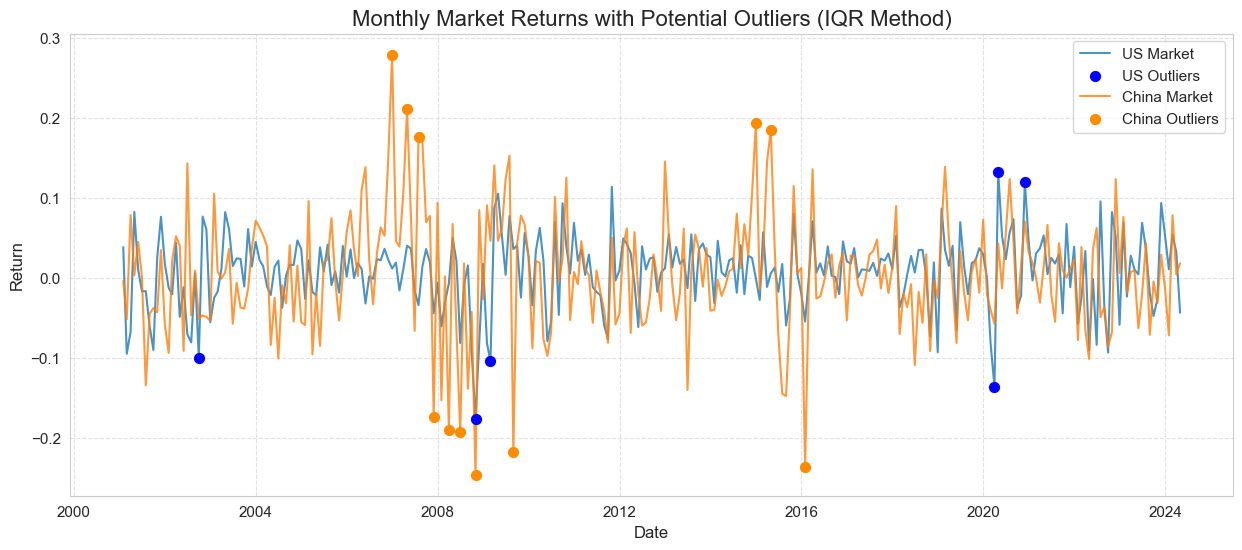
\includegraphics[width=5in]{figures/outliers/Market Outliers.png}
\caption{Monthly Market Returns with Potential Outliers}
\label{fig:label7}
\end{center}
\end{figure}

\subsubsection{Economic Outliers}

Theme values in the U.S. and China were also analyzed for outliers using the IQR method. Figure~\ref{fig:label8} shows box plots of the themes for each country, measured at the monthly granularity. The plot reveals some similarities in theme variance across the countries, but it also reveals great differences in others. Accruals Debt Issuance, Profit Growth, and Seasonality were among the most compact Themes for both countries. Momentum was one of the most varying themes, with severe outliers in both countries. Size was the most varied data in the Chinese economy, though much more stable in the U.S. economy. Most other factors were generally more varied in the Chinese economy than the U.S. economy.

\begin{figure}[htbp]
\begin{center}
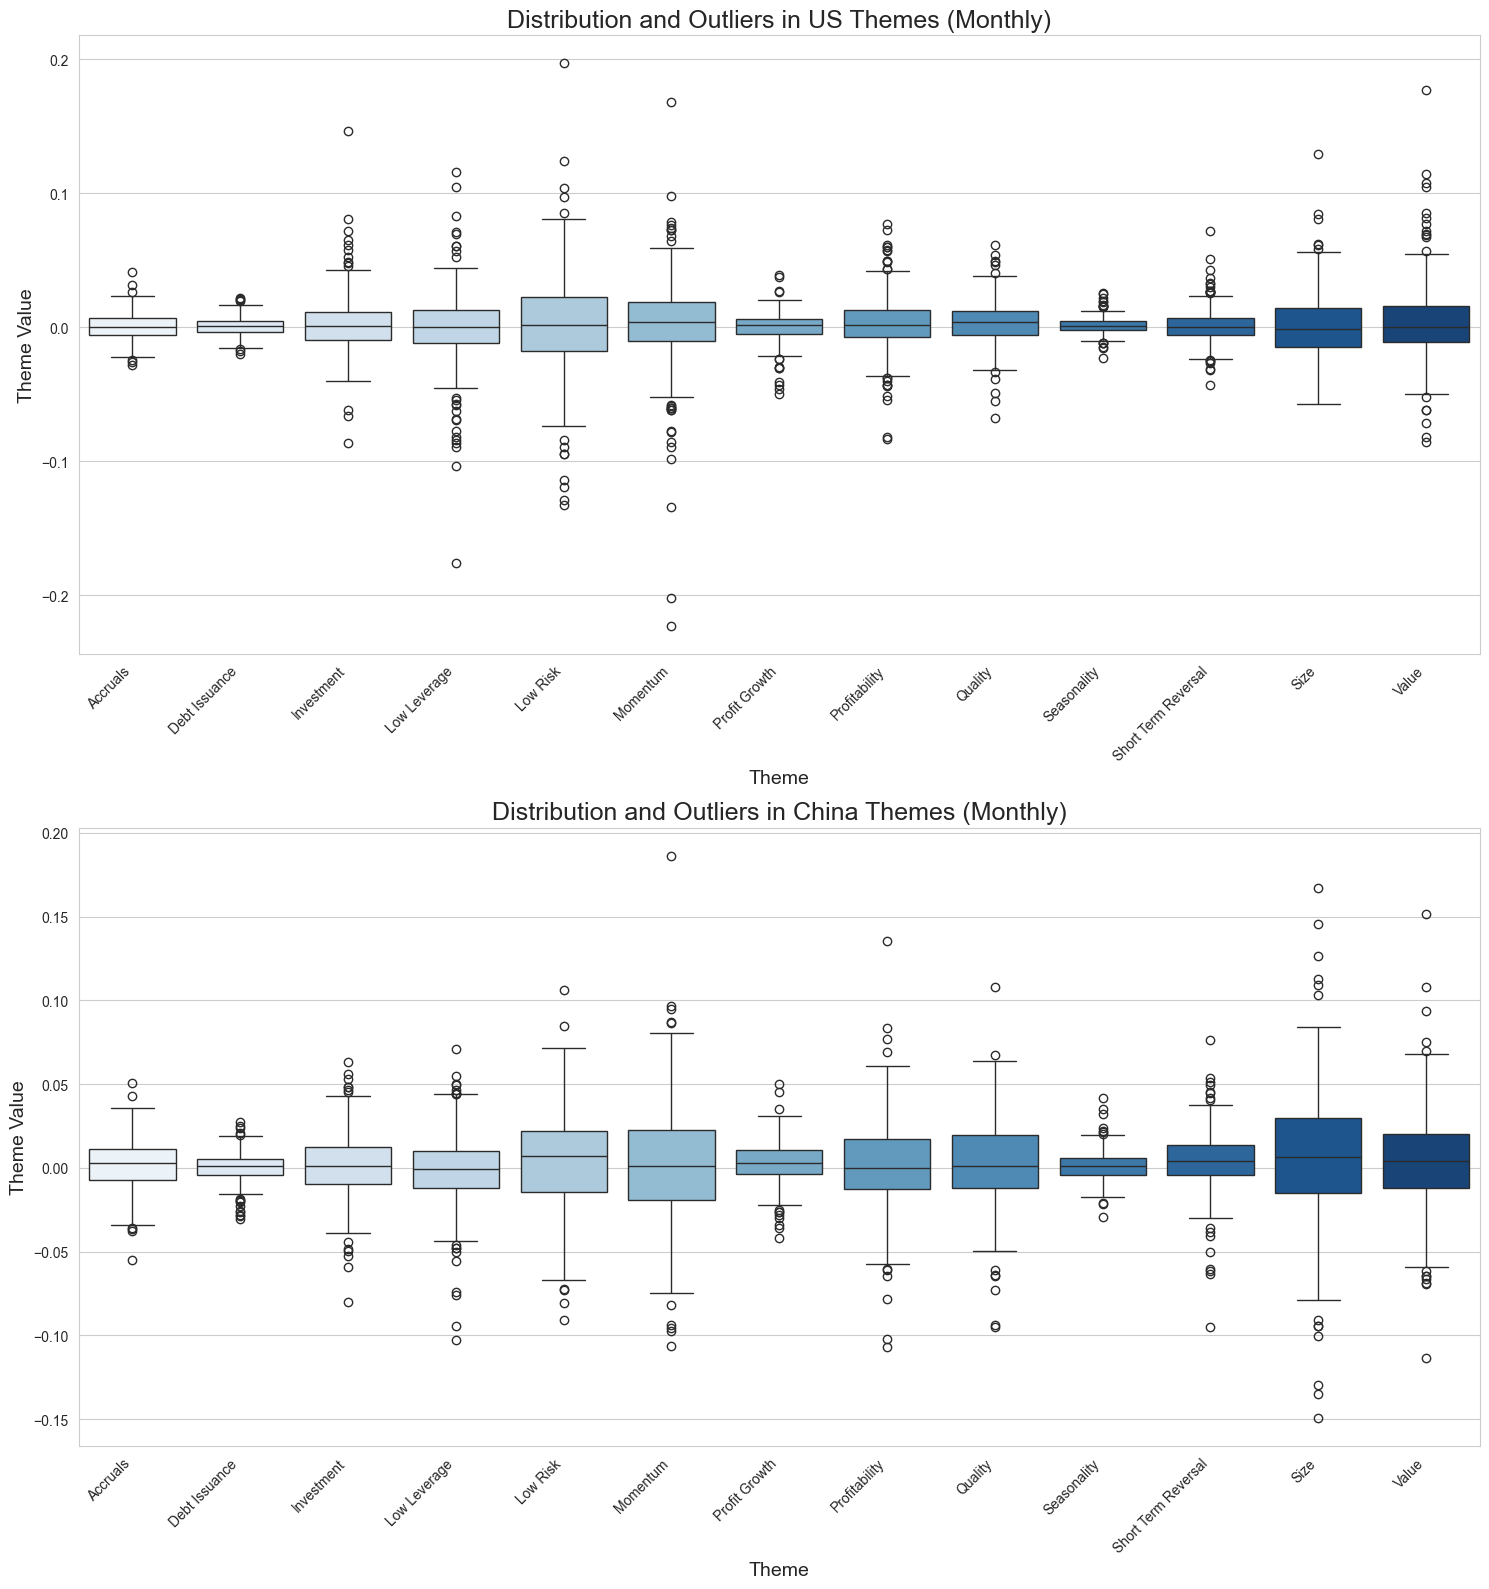
\includegraphics[width=5in]{figures/outliers/Theme Outliers Boxplots.png}
\caption{Box Plots of U.S. and China Themes}
\label{fig:label8}
\end{center}
\end{figure}

Theme and factor volatilities were calculated as 6-month rolling standard deviations for all columns, either all themes or all factors, for each country and then averaged. Examining the results, we see similar trends over time for themes and factors. Theme volatilities are placed in the appendix (see Figure~\ref{fig:label9}). Figure~\ref{fig:label10} shows the factor volatilities over time for the U.S. and Chinese economies. It confirms our suspicions of the Chinese economy generally having a greater volatility than the U.S. economy, and it shows periods of divergence and near-convergence of the volatilities. Most recently, the volatilities have generally been the same since 2020. 

\begin{figure}[htbp]
\begin{center}
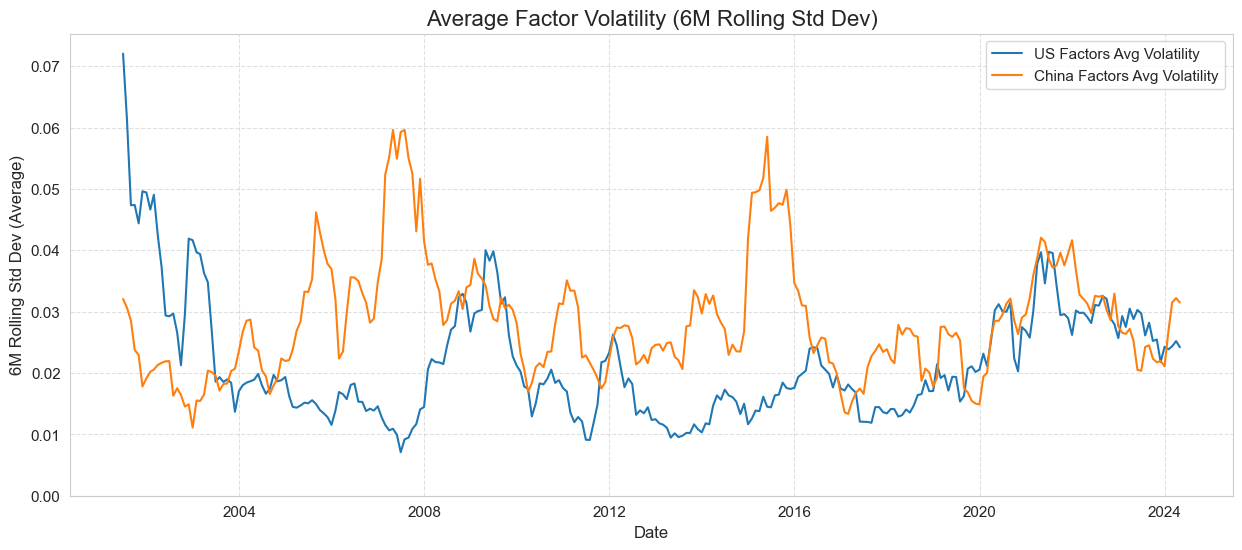
\includegraphics[width=5in]{figures/outliers/Average Factor Volatility Rolling SD.png}
\caption{Factor Volatility (6-Month Rolling Standard Deviation)}
\label{fig:label10}
\end{center}
\end{figure}

I also examined the number of outliers over time in each country for factors and months. The results were consistent with the volatilities above, with areas with greater volatility having more outliers. The plot of the number of factor outliers over time is shown in Figure~\ref{fig:label11}, and the plot of the number of theme outliers over time is shown in Figure~\ref{fig:label12}. We note that it is very rare for factors and themes to have no outliers at a given time point.

When deciding what to do with outliers, we have a few options. We can retain outliers, using the data as it appears. These cases do not appear to be miscalculations or as a result of human error; they align with historically significant scenarios. Keeping the data can impact the result of the models, especially models that use MSE as an objective function. Significant scenarios in either country might significantly impact the regression. As a result, one potential method would be to fit a model on the entire 2001 to 2024 region, and then again post-2010 for more recent events; still, the models would likely be influenced by the 2015 bubble in the Chinese market.

We can exclude the outliers, following some criteria for when to include or exclude a time period. However, these outliers are not errors and are not irrelevant to the relationship between the markets. Excluding outliers or idiosyncratic scenarios biases the models by omitting important market scenarios. 

We can winsorize outliers to reduce their impact. We might set any data above the 99th percentile to be the same value as the 99th percentile (and similarly for the 1st percentile). This complicates the interpretation of the effect size and does not exclude the impact of the outliers in the models. 

As a result, I've chosen to winsorize the all columns in the data at the 0.05\% and 99.95\% levels. In the monthly data, this will impact 1.430\% of the cells in the factors dataset, 1.429\% of the cells in the themes dataset, and 1.429\% of the cells in the returns dataset. For the daily data, it will impact 1.021\% of the cells in the factors dataset, 1.021\% of the cells in the themes dataset, and 1.21\% of the cells in the returns dataset. In total, 

This choice was made in order to limit the impact of extreme values in the data. It's important to note that it still preserves the information from the outliers, but it caps the amount of effect a single point can have. The literature also shows that this does not fully eliminate outlier bias, showing that the signals of the winsorized outliers remain. 

\subsection{Standardizing the Data}

Applying the Shapiro test for normality at an $\alpha=0.05$ level shows that none of the columns in the daily data is normal or standardized. Of the monthly datasets, no columns are standardized, but 34 of the 262 factor columns are normal and 4 of the 28 theme columns are normal. I checked for standardization in the data by checking if the mean of a column's data $\mu$ satisfies $|\mu|\leq 0.05$ and its standard deviation $\sigma$ satisfies $0.95\leq \sigma\leq 1.05$.

The themes and factors are standardized as follows using sklearn's StandardScaler. Suppose that $x_{i,j}$ represents the value of row $i$ in column $j$. Let $\mu_j$ and $\sigma_j$ be the mean and standard deviation of the data in column $j$. The standardized value of $x_{i,j}$, denoted as $x_{i,j}^{(std)}$, is given by $x_{i,j}^{(std)}=\frac{x_{i,j}-\mu_j}{\sigma_j}$.

Note that, as outlined in the statistical formulation of the models, the factors and themes are not assumed to be normally distributed. As such, standardizing the data is enough.

\subsection{Stationarity and Structural Breaks}

\subsubsection{Testing for Stationarity and Structural Breaks}

As described in the statistical formulation section, stationarity is an important assumption of the models Two tests are used to assess stationarity: the Augmented Dickey-Fuller (ADF) Test and the Kwiatkowski-Phillips-Schmidt-Shin (KPSS) Test. I used both at the $\alpha=0.05$ level.

The ADF test has the null hypothesis that the time series is non-stationary, and an alternative hypothesis that it is. It can be implemented using adfuller() from statsmodels in Python. The series is said to be stationary when the null is rejected when the p-value is less than 0.05.

The KPSS test has the null hypothesis that the time series is stationary, and an alternative hypothesis that it is not. It can be implemented using kpss() from statsmodels in Python. The series is said to be stationary when we fail to reject the null hypothesis, when the p-value is greater than 0.05.

In order to detect structural breaks in the data, the Pruned Exact Linear Time (PELT) algorithm is also used. It detects multiple change points in time series data, and it can be implemented using the ruptures package. It efficiently searches for optimal segmentation using the squared error cost function. 

The time series were plotted with vertical lines marking detected break points.

I also used the CUSUM (Cumulative Sum) test for breaks in the US-China relationship, which looked for structural changes in regression relationships between the market returns.

\subsubsection{Testing Results}

In the monthly factors dataset, the ADF test concluded that 261 of the 262 columns were stationary and the KPSS test concluded that 240 of the 262 columns were stationary. They both agreed on 239 columns being stationary. Using the CUSUM test, a break was detected in the relationship, with $p<0.0001$. 

In the monthly themes dataset, the ADF test concluded that 27 of the 28 columns were stationary and the KPSS test concluded that 26 of the 28 columns were stationary. They both agreed on 25 columns being stationary. Using the CUSUM test, a break was detected in the relationship, with $p=0.0002$. 

In the daily factors dataset, the ADF test concluded that all 262 columns were stationary and the KPSS test concluded that 197 of the 262 columns were stationary. Using the CUSUM test, a break was detected in the relationship, with $p<0.0001$.

In the daily themes dataset, the ADF test concluded that all 28 columns were stationary and the KPSS test concluded that 22 of the 28 columns were stationary. Using the CUSUM test, a break was detected in the relationship, with $p<0.0001$.

Structural breaks were analyzed in the factors and themes as well, at both the daily and monthly granularities. Two  common trends amongst those with structural breaks were in the middle of 2002 and in 2022.

\subsubsection{Making the Data Stationary}

While every column in the data was described as stationary by at least one of the tests, I decided to only count data as stationary if both models agree on it. As such, there were 97 columns that needed to be changed in some way.

I wrote a function that attempted a few transformations, checking for stationarity as it applied different ones. First, it attempts differencing, in which observations are subtracted from their previous values. This is generally great for series with upward or downward trends. If that doesn't work, the natural logarithm is used instead; this accounts for exponential growth in the data. The square root transformation is attempted next. Lastly, the Box-Cox and Yeo-Johnson transformations are attempted, which normalize the data. Lastly, the function standardizes any data it is able to make stationary.

In the monthly factors data, 23 columns were identified as non-stationary by either test. Of those, 21 were transformed into stationary columns, 20 by differencing and 1 using the Yeo-Johnson transformation. The two columns that didn't achieve stationarity by any method were usa\_factors\_monthly\_aliq\_mat and chn\_factors\_monthly\_age.

In the daily factors data, 65 columns were identified as non-stationary by either test. Of those, 61 were transformed into stationary columns, 59 by differencing and 2 using the Yeo-Johnson transformation. The four columns that didn't achieve stationarity by any method were usa\_factors\_daily\_lnoa\_gr1a, chn\_factors\_daily\_ocf\_at, usa\_factors\_daily\_fnl\_gr1a, and usa\_factors\_daily\_nncoa\_gr1a.

In the monthly theme data, 3 columns were identified as non-stationary by either test. All three were transformed into stationary columns by differencing. In the daily theme data, 6 columns were identified as non-stationary by either test. All six were transformed into stationary columns by differencing.

\subsubsection{The Cumulative Sum Test on Market Returns}

The cumulative sum (CUSUM) test is a technique used to detect structural breaks or regime shifts in financial data. It looks at the cumulative sum of deviations from a target value. When it exceeds the target value, it signals a change in the underlying process. 

The U.S. results, shown in Figure~\ref{fig:label16}, reveal a few potential structural breaks: 2001, 2007-2008, and 2011-2013. The China results, shown in Figure~\ref{fig:label17}, reveal a few other potential structural breaks: 2001, 2007-2009, and 2015. These results align with the historical contexts presented earlier in the thesis.

\begin{figure}[htbp]
\begin{center}
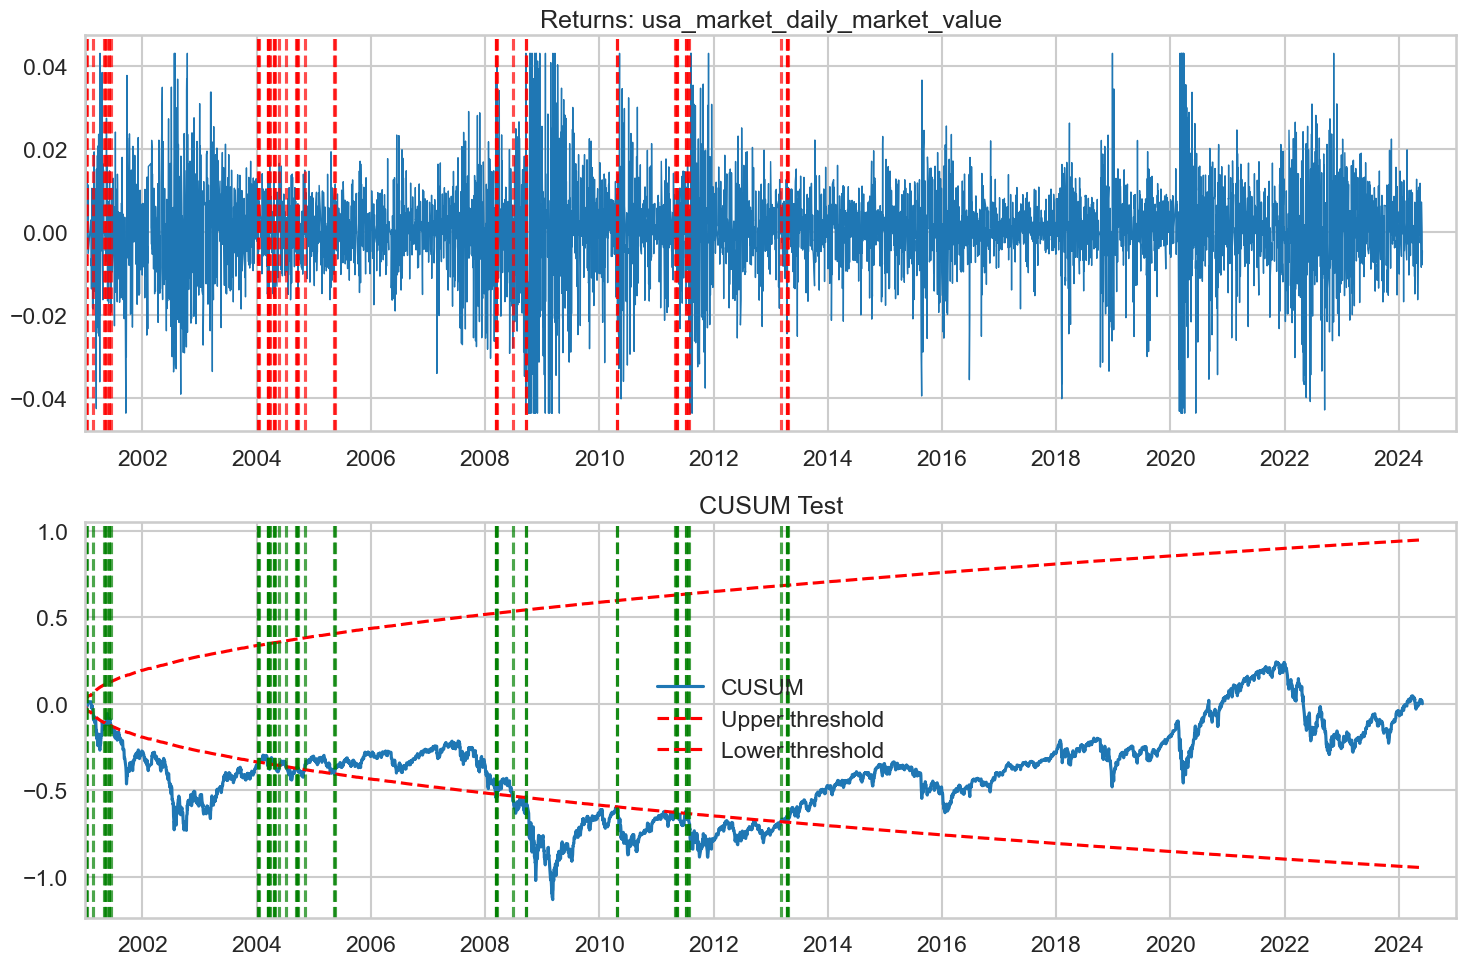
\includegraphics[width=4in]{figures/stationarity/US CUSUM Test.png}
\caption{CUSUM Test on U.S. Market Returns}
\label{fig:label16}
\end{center}
\end{figure}


\begin{figure}[htbp]
\begin{center}
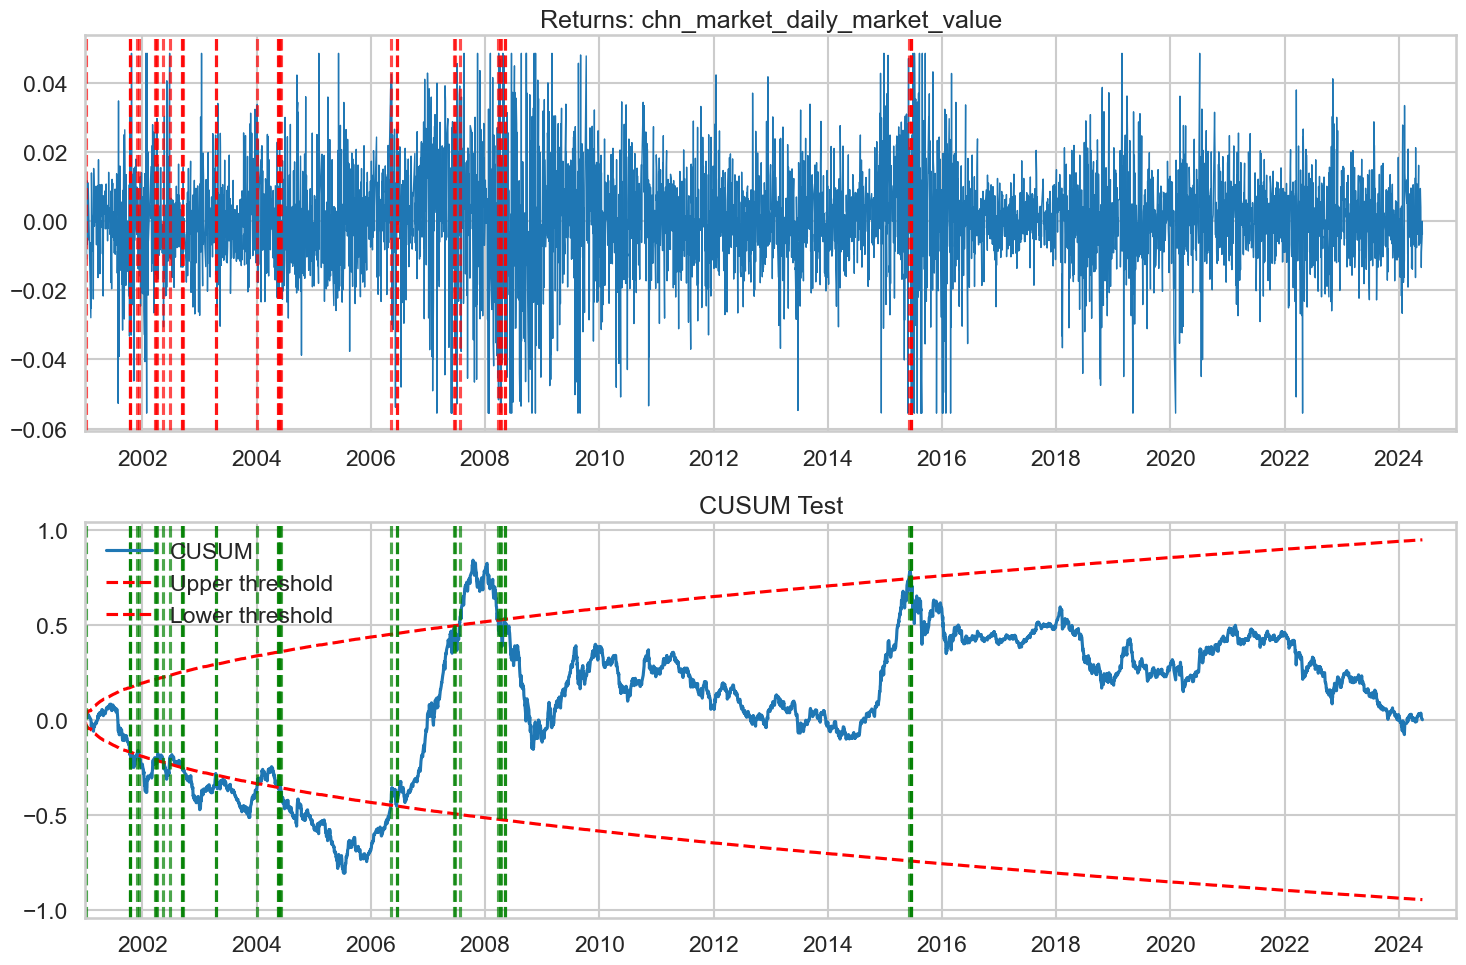
\includegraphics[width=4in]{figures/stationarity/China CUSUM Test.png}
\caption{CUSUM Test on Chinese Market Returns}
\label{fig:label17}
\end{center}
\end{figure}

\subsection{Limitations in the Data}

There are a few considerations we must take when analyzing the data with our models. First, stationarity was resolved in some factors, but those will likely pose an issue with interpretation. Second, some factors were removed due to data missingness and a lack of stationarity, even after attempting transformations. Lastly, there are some issues with structural breaks in the markets, typically representative of shifts in regimes or policy. With the lastest structural break being a decade ago, we can still analyze the integration from 2016-2024.